\chapter{Desenvolvimento da solução}
	\label{ch:desenvolvimento}
Neste capítulo é discutido sobre o desenvolvimento do \textit{software} de tratamento de dados proposto por este trabalho. 

O programa feito para receber as informações provindas do veículo é implementado em sua totalidade na linguagem interpretada Python v3.6, esta foi escolhida devido a facilidades que a mesma proporciona no uso de bibliotecas de suporte ao sistema e de interfaceamento gráfico além de ser uma linguagem comum ao autor. Outras linguagens como o C++ foram consideras para a aplicação, porém como o fluxo de dados não é feito em grande escala a velocidade de processamento não é uma questão primária. O sistema que atua no microcontrolador é programado em C e C++, pois este é o padrão de desenvolvimento para os microcontroladores utilizados. 

\section{Bibliotecas e Softwares utilizados}
O sistema de tratamento de dados utiliza de diversos recursos disponíveis na linguagem Python sejam eles bibliotecas ou até mesmo \textit{frameworks}, a seguir é discutido sobre tais recurso e como são utilizados no sistema. 

Um dos principais componentes do \textit{software} é a interface gráfica, ou interface do usuário. É por meio dela que a equipe presente nos boxes pode ter acesso as informações do veículo, observando os gráficos de tração, velocidade, extensometria, etc... Para a concepção da interface gráfica foi utilizada um \textit{framework} chamada Qt \footnote[1]{Site: \url{https://www.qt.io/}}. O Qt é nativamente utilizado para o C++ na construção de interfaces gráficas, para utilizar-lo no Python, é necessário a utilização de uma biblioteca auxiliar chamada PyQt\footnote[2]{URL: \url{https://riverbankcomputing.com/software/pyqt/intro}}. Tanto o Qt quanto o PyQt estão disponíveis em Windows, distribuições Linux e MacOS, um fator importante visto que a equipe utiliza o sistema operacional Windows, porém o autor desenvolveu o sistema utilizando a distribuição Manjaro XFCE e Ubuntu 16.04. Este é um tema recorrente neste trabalho, todas as bibliotecas utilizadas devem ser portáveis para ambos os sistemas operacionais Windows ou distribuições Linux como declarado nos objetivos específicos. As versões utilizadas das bibliotecas foram o Qt 5.5.1 e o PyQt 5

Para o desenvolvimento foi utilizada a ferramenta Designer da \textit{framework} Qt. A ferramenta permite a criação de telas com auxílio de interface gráfica e após a construção das mesmas telas, se utiliza um comando de linha (\textit{pyuic5}) para transformar o código bruto da tela de XML para Python. Este novo código em Python é utilizado para se referenciar os objetos dentro da interface, necessário para união da parte lógica com a parte gráfica.

Uma característica específica deste sistema é a execução da parte gráfica em paralelo a recepção de dados. Isto implica que a parte gráfica deve ser executada em conjunto com o recebimento dos dados enviados pelo veículo, tendo isto em mente, é necessário utilizar de processamento paralelo para fazer ambas as tarefas. A solução encontrada para tal foi a biblioteca \textit{multiprocessing} do Python. Esta biblioteca possui funções para criação de \textit{pipes}, estrutura que retorna dois objetos representando um "tubo" de passagem de informação entre dois processos, ambos os processos tem acesso a comandos de envio e recepção de dados para conversa entre duas aplicações em tempo real. A função \textit{pipe} opera de forma \textit{duplex}, onde ambos os lados podem enviar e receber dados, porém devido ao escopo atual do projeto o sistema será utilizado como \textit{simplex}.    

Para a conexão do sistema de boxes com o microcontrolador é utilizado o protocolo de rede sem fio ZigBee. O protocolo é definido como uma solução para sistemas de baixa taxa de transmissão de dados e baixo consumo de energia, ele opera no alcance de uma PAN e tem uma taxa de transferência de até 250Kbps \cite{elahi2009zigbee}. Estas características e outras informações revisadas na Seção \ref{sec:zigbee} levaram a utilização deste protocolo para a comunicação sem fio entre os sistemas citados. Para realizar o processamento dos pacotes recebidos pelo módulo ZigBee no computador foi utilizada a biblioteca \textit{python-xbee}. Esta biblioteca permite ler e escrever pacotes para os módulos que estão na rede PAN sem necessidade de utilizar comandos diretos para as entradas da porta USB. Para utilizar a biblioteca é configurado o \textit{baud rate} e qual entrada está localizado o modulo ZigBee. 

Um \textit{software} auxiliar foi utilizado para a configuração dos módulos ZigBee. O XCTU\footnote[3]{URL: \url{https://www.digi.com/products/xbee-rf-solutions/xctu-software/xctu}} faz a configuração inicial entre os módulos a fim de ordenar quem terá qual papel na rede. Além de configurar quem será o coordenador e quem será o roteador/\textit{end-point}, o XCTU também configura qual será o ID da PAN, em qual modo o módulo irá operar seja ele API ou AT, permite envio de pacotes de teste entre os envolvidos e também de sequencias de pacotes. 

\section{Hardware utilizado}
\label{sec:hardwareutilizado}

Para o desenvolvimento do sistema foram utilizados alguns equipamentos de \textit{hardware}. Devida a proposta de solução foi necessária a utilização de alguns equipamentos específicos para o desenvolvimento do sistema , estes equipamentos utilizados no sistema são listados a seguir:

\begin{itemize}
	\item Xbee ZigBee PRO series 2;
	\item Xbee ZigBee series 2;
	\item XBee Explorer USB Adapter;
	\item Arduino Nano V3;
	\item Sensores automotivos;
	\item \textit{Shield} para acoplar as placas;e
	\item Computador para receber os dados. 
\end{itemize}  

Os módulos Xbee ZigBee series 2/PRO series 2 \cite{xbeeuserguide} foram adicionados no decorrer do projeto. A telemetria foi uma das aspirações iniciais desse trabalho de conclusão de curso, porém devido ao tamanho do escopo do projeto a execução desta parte do sistema foi retirada. Contudo durante as reuniões feitas em conjunto com o sub-sistema de eletrônica veicular do Baja Velociraptor, foi decidido que a telemetria entraria no escopo anual do projeto 2018 do veículo. Com a entrada deste projeto, alguns dos membros se comprometeram a ajudar na construção desse sistema e também na compra dos módulos para uso do protocolo ZigBee. Tendo todo este cenário, foi decidido entre o autor e orientador pela opção de produção deste sistema pronto para receber dados via telemetria, no qual o sistema que adquire os dados é executado ao mesmo tempo que o sistema que trata esses mesmos dados. 

Em relação ao módulo utilizado, ele possui as características base do protocolo ZigBee porém a versão comprada (PRO) possui algumas característica melhoradas. Por exemplo: O alcance urbano do Xbee ZigBee series 2 é de 40 metros, já da versão PRO é de 90 metros, o alcance em área rural/aberta, com pouca interferência de sinal, é de 120 metros na versão padrão e 3.200m na versão PRO \cite{xbeespecs}. Para a realizão dos testes foram utilizados um modulo Xbee ZigBee series 2 e um Xbee ZigBee PRO series 2, ambos são compatíveis sem necessidade de uso de bibliotecas auxiliares ou modificação de \textit{firmware}.

O Xbee Explorer USB Adapter\footnote[1]{URL: \url{https://www.filipeflop.com/produto/xbee-explorer-usb-adapter/}} é um adaptador USB para utilizar o módulo ZigBee ligado direto aos computadores para configurar. Ele permite a utilização do \textit{software} XCTU de forma eficiente, sem a necessidade de conectar o módulo ZigBee a um outro módulo FTDI\footnote[2]{URL: \url{http://www.ftdichip.com/}}, que faz conexão com o computador. 

O Arduino Nano V3 foi utilizado por ser mais prático de realizar os testes, as configurações desta placa de desenvolvimento são as mesmas apresentadas na Seção \ref{sec:placasdedesenvolvimento}. Nenhuma biblioteca exclusiva das plataformas Arduino foi utilizada para enviar os dados do microcontrolador para o computador. O módulo Xbee ZigBee recebe os dados tratados e envia para a outra ponta de forma serial pelos pinos \textit{Rx} e \textit{Tx}, a outra ponta dos dados deve se receber os mesmos e tratar-los de acordo com o protocolo.

O computador utilizado nos testes possui um processador Intel I5 7200U e 8GB de memória RAM. Estes são os atributos de maior relevância para a execução do sistema já que os dados são recebidos diretamente dos módulos ZigBee e apenas gravados em HD no formato de gráficos. Na Figura \ref{fig:sistemapronto} é demonstrado o sistema embarcado no veículo, pronto para transmitir os dados dos testes realizados no Capítulo \ref{ch:testes}. 

\begin{figure}[!htb]
	\centering
		\caption{Sistema de controle \textit{on-board} montado no veículo.}
		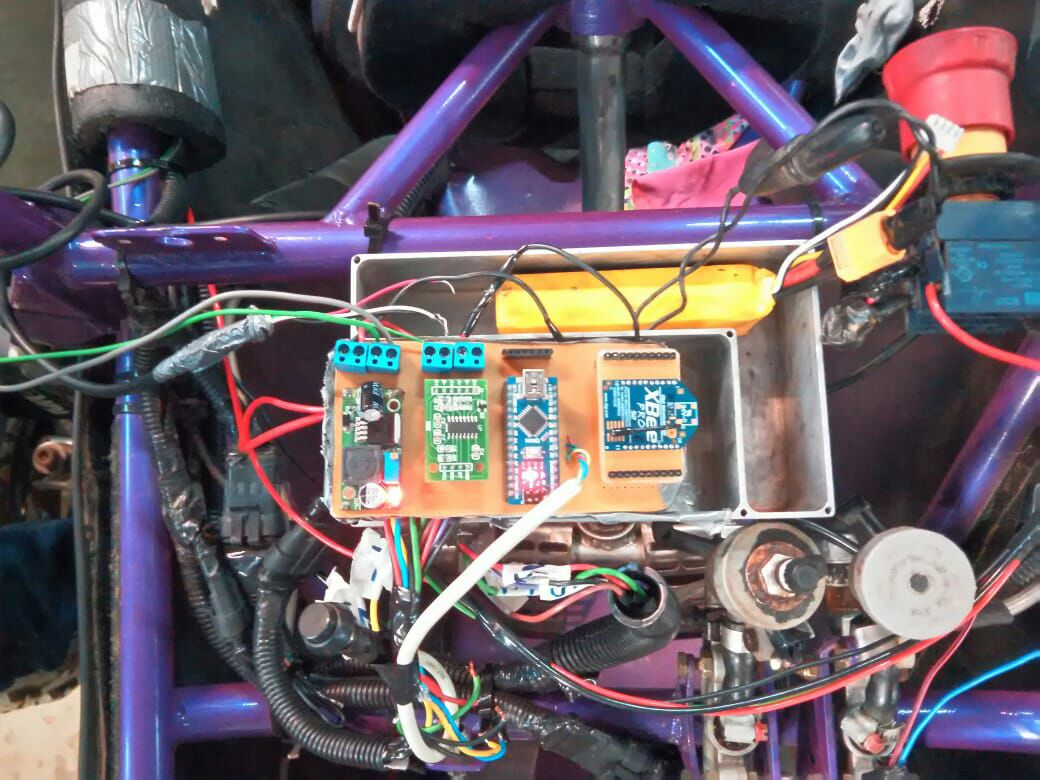
\includegraphics[scale=0.3]{sistemapronto} 
		\caption*{Fonte: Autor.}
		\label{fig:sistemapronto}
\end{figure}    


\section {Software desenvolvido}
Nesta seção será apresentado o \textit{software} que foi criado para tratamento dos dados provindos do veículo. Na seção será demonstrada tela a tela quais são as funcionalidades do sistema.

Inicialmente temos a tela principal na Figura \ref{fig:telaprincipal}. Nela é possível ir para as outras telas de funcionalidades do sistema na barra superior, além de ter as funcionalidades padrões para provas de enduro, uma das modalidades dos campeonatos de baja SAE. Na região superior direita é possível visualizar o contador do nível do combustível, ele inicia em 8 marcações quando o tanque está cheio e progride até 0 quando o tanque de combustível está vazio. No canto inferior direito estão presentes os alertas importantes para a equipe durante a prova, entre os alertas existem o de temperatura do motor que é ligado quando o óleo do mesmo passa de 125$^\circ$C, o de extensometria que é acionado quando algum ponto do chassis sofre um esforço de tensão maior do que um valor \textit{X} e o da bateria que é acionado quando a corrente da bateria está baixa. No canto inferior esquerdo está disposto os dados de velocidade do veículo em quilômetros por hora e a temperatura do motor na ultima coleta de dados. Por último no canto superior esquerdo é disposta a tabela de dados de volta, onde a cada volta são mostrados os dados de número da volta, tempo de volta e combustível restante após a mesma. 

\begin{figure}[!htb]
	\centering
		\caption{Tela principal do programa.}
		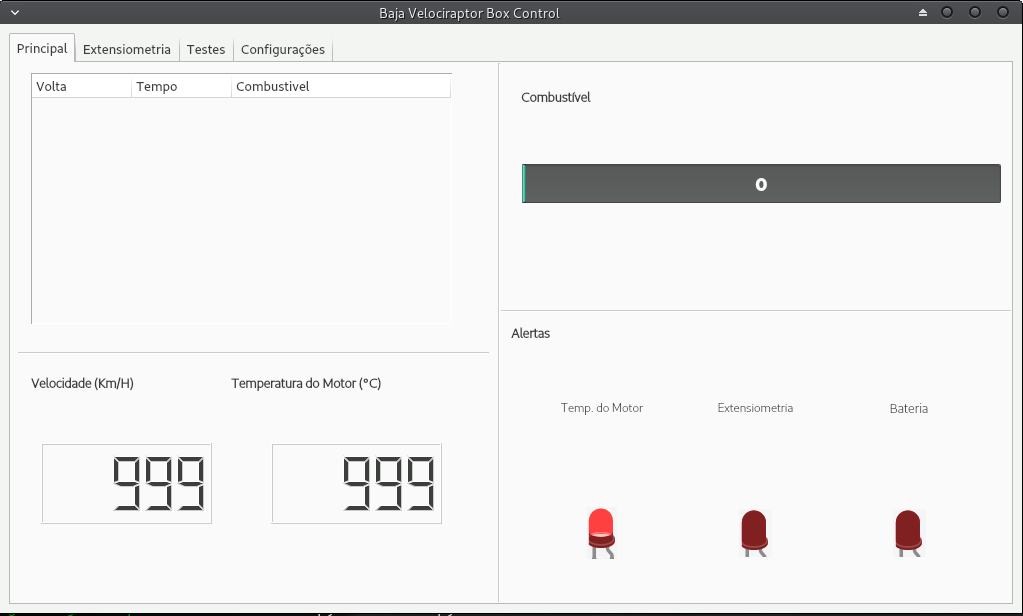
\includegraphics[scale=0.4]{telaprincipal} 
		\caption*{Fonte: Autor.}
		\label{fig:telaprincipal}
\end{figure}    

A segunda tela possui as informações da extensometria. Estes dados são provindos de quatro sensores espalhados no carro que dão informação sobre a torção exercida sobre o chassis em aceleração, saltos e curvas. A Figura \ref{fig:telaextensometria} demonstra essa tela.

\begin{figure}[!htb]
	\centering
		\caption{Tela de extensometria.}
		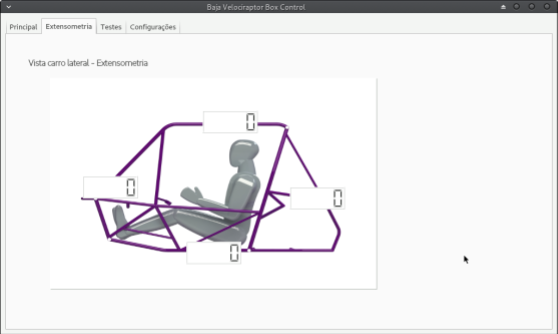
\includegraphics[scale=0.4]{telaextensometria} 
		\caption*{Fonte: Autor.}
		\label{fig:telaextensometria}
\end{figure}    

A tela da Figura \ref{fig:telatestes} possui as opções de gráficos que se deseja visualizar. O principal objetivo é gerar gráficos para o monitoramento do veículo em testes ou em prova. O gráfico de força de tração tem como foco os testes do veículo, já os de velocidade/RPM, temperatura do motor e de nível do combustível são utilizados em tempo de prova. Mais de um gráfico pode ser aberto ao mesmo tempo, acrescentando modularidade a disposição das telas, a Figura \ref{fig:telagrafico} exibe um exemplo de como o gráfico é gerado, os dados são provenientes do veículo.

\begin{figure}[!htb]
	\centering
		\caption{Tela de seleção de gráficos de teste e monitoramento.}
		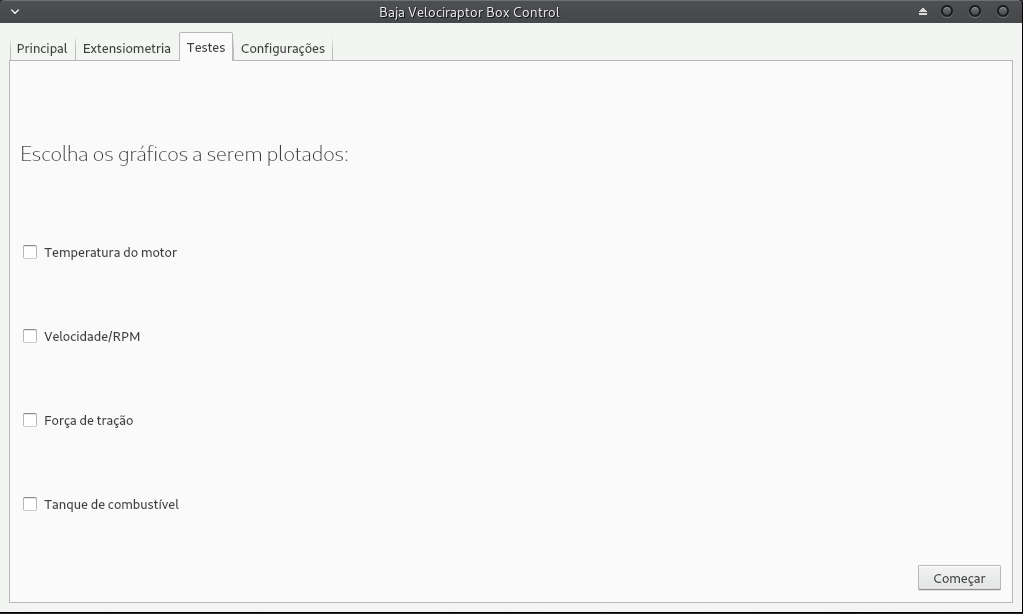
\includegraphics[scale=0.4]{telatestes} 
		\caption*{Fonte: Autor.}
		\label{fig:telatestes}
\end{figure}    

\begin{figure}[!htb]
	\centering
		\caption{Tela com exemplo de gráfico de temperatura do motor por tempo em segundos.}
		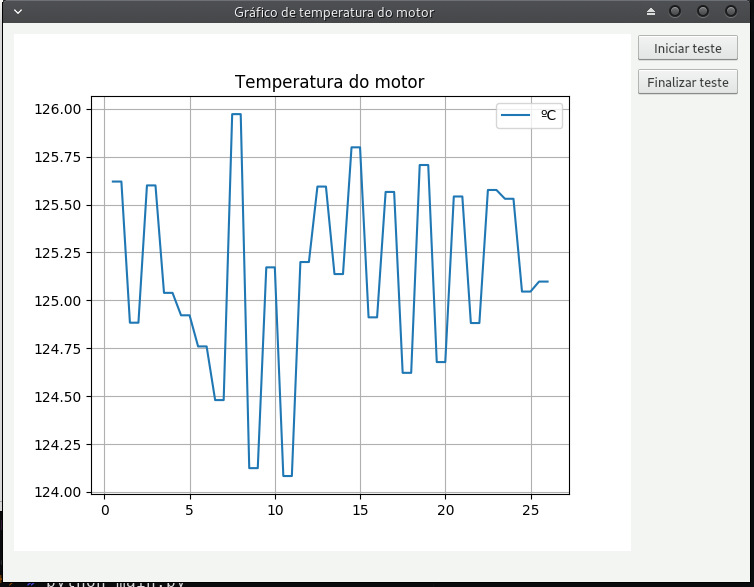
\includegraphics[scale=0.4]{telagrafico} 
		\caption*{Fonte: Autor.}
		\label{fig:telagrafico}
\end{figure}    

Por ultimo a Figura \ref{fig:telaconfiguracao} exibe as configurações do sistema. Atualmente a única opção é desligar o sistema, fechando as portas, \textit{pipes} e processos abertos. Estas são as telas presentes nos programas, elas foram construídas em conjunto com a equipe Velociraptor para atender as demandas geradas pelos sensores presentes nos veículos.


\begin{figure}[!htb]
	\centering
		\caption{Tela de configurações.}
		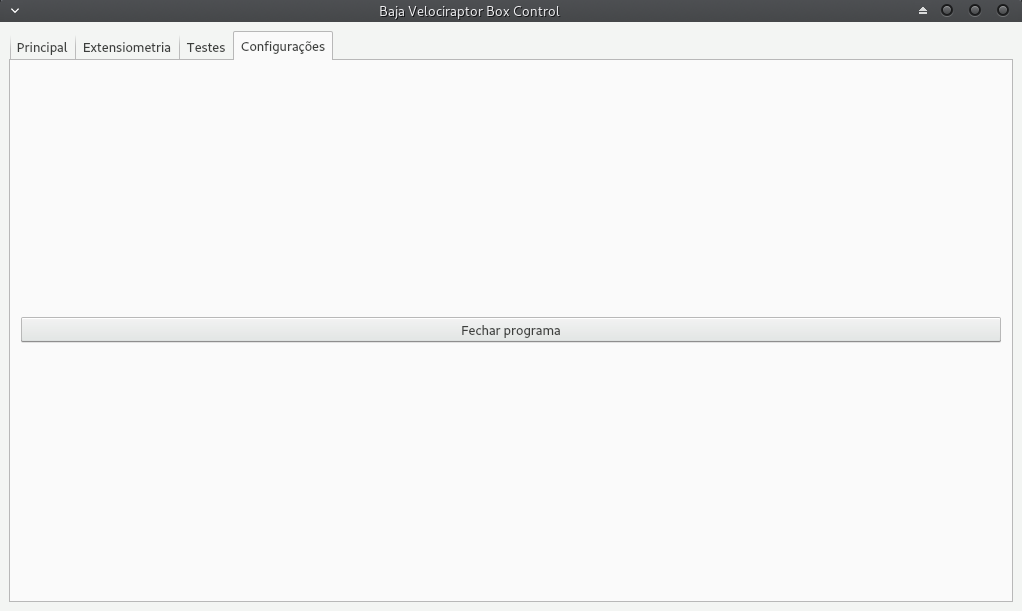
\includegraphics[scale=0.4]{telaconfiguracoes} 
		\caption*{Fonte: Autor.}
		\label{fig:telaconfiguracao}
\end{figure}    

